\chapter{REVIEW OF LITERATURE}

\section{Overview}
Human Pose Estimation (HPE) is a fundamental task in computer vision that aims to localize anatomical keypoints (such as joints and limbs) from images or video sequences. Over the last two decades, HPE research has transitioned from rule-based graphical models and manual feature descriptors (such as Histogram of Oriented Gradients) to deep convolutional neural networks. This chapter surveys key literature and technology frameworks relevant to real-time posture tracking, sequence classification, and high-performance web deployment.

\section{Markerless Human Pose Estimation}
Traditional motion capture systems rely on reflective markers and multi-camera arrays. While highly accurate, these systems are prohibitively expensive, require extensive setup, and are limited to laboratory environments. Markerless pose estimation offers an accessible alternative. 

Early deep learning approaches like DeepPose (Toshev et al., 2014) formulated keypoint localization as a regression problem. Subsequent networks, such as Stacked Hourglass Networks (Newell et al., 2016) and OpenPose (Cao et al., 2017), utilized heatmap regression to estimate joint locations with high accuracy. Although OpenPose supports multi-person detection, its heavy multi-stage architecture requires high-end server GPUs, rendering it unsuitable for real-time edge execution on average customer laptops or mobile devices.

\section{MediaPipe Pose Framework}
To address the need for low-latency, mobile-compatible pose estimation, Google developed the MediaPipe framework (Lugaresi et al., 2019). The framework provides modular machine learning pipelines that process media inputs (video, audio) in real-time.

At the core of MediaPipe's pose tracking is the BlazePose model (Bazarevsky et al., 2020), which is designed specifically for single-person fitness and dance applications. BlazePose utilizes a two-stage detector-tracker topology:
\begin{enumerate}
    \item \textbf{Pose Detector:} A lightweight convolutional network locates the region of interest (ROI) and identifies the person's bounding box and alignment parameters. This detector runs only when tracking is lost, saving computation.
    \item \textbf{Pose Tracker:} A regression network predicts the 3D coordinates of 33 landmarks and a visibility score for each point.
\end{enumerate}
BlazePose outputs 33 coordinates based on the topology shown in Figure 2.1, including standard joints (elbows, knees, wrists) as well as facial features (eyes, nose, mouth) and feet landmarks. By running inference on local GPU hardware via WebGL or C++ bindings, MediaPipe achieves real-time execution speeds of over 30 FPS on standard edge devices.

\begin{figure}[h]
\centering
% Drawing a simple schematic of MediaPipe Pose skeleton using TikZ
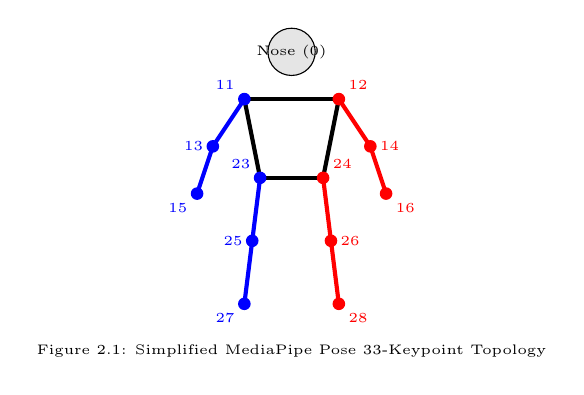
\begin{tikzpicture}[scale=2]
  % Head
  \draw[fill=gray!20] (0,0.8) circle (0.15);
  \node[font=\tiny] at (0,0.8) {Nose (0)};
  % Torso
  \draw[line width=1.5pt] (-0.3,0.5) -- (0.3,0.5); % Shoulders
  \draw[line width=1.5pt] (-0.2,0) -- (0.2,0); % Hips
  \draw[line width=1.5pt] (-0.3,0.5) -- (-0.2,0); % Left Torso
  \draw[line width=1.5pt] (0.3,0.5) -- (0.2,0); % Right Torso
  
  % Left Arm
  \draw[line width=1.5pt, blue] (-0.3,0.5) -- (-0.5,0.2) -- (-0.6,-0.1);
  \fill[blue] (-0.3,0.5) circle (0.04) node[above left, font=\tiny] {11};
  \fill[blue] (-0.5,0.2) circle (0.04) node[left, font=\tiny] {13};
  \fill[blue] (-0.6,-0.1) circle (0.04) node[below left, font=\tiny] {15};
  
  % Right Arm
  \draw[line width=1.5pt, red] (0.3,0.5) -- (0.5,0.2) -- (0.6,-0.1);
  \fill[red] (0.3,0.5) circle (0.04) node[above right, font=\tiny] {12};
  \fill[red] (0.5,0.2) circle (0.04) node[right, font=\tiny] {14};
  \fill[red] (0.6,-0.1) circle (0.04) node[below right, font=\tiny] {16};
  
  % Left Leg
  \draw[line width=1.5pt, blue] (-0.2,0) -- (-0.25,-0.4) -- (-0.3,-0.8);
  \fill[blue] (-0.2,0) circle (0.04) node[above left, font=\tiny] {23};
  \fill[blue] (-0.25,-0.4) circle (0.04) node[left, font=\tiny] {25};
  \fill[blue] (-0.3,-0.8) circle (0.04) node[below left, font=\tiny] {27};

  % Right Leg
  \draw[line width=1.5pt, red] (0.2,0) -- (0.25,-0.4) -- (0.3,-0.8);
  \fill[red] (0.2,0) circle (0.04) node[above right, font=\tiny] {24};
  \fill[red] (0.25,-0.4) circle (0.04) node[right, font=\tiny] {26};
  \fill[red] (0.3,-0.8) circle (0.04) node[below right, font=\tiny] {28};

  \node[align=center, font=\tiny] at (0,-1.1) {Figure 2.1: Simplified MediaPipe Pose 33-Keypoint Topology};
\end{tikzpicture}
\caption{MediaPipe Pose Keypoint Mapping.}
\label{fig:mediapipe_topology}
\end{figure}

\section{Deep Learning Sequence Classification}
While frame-by-frame joint angle calculation works for static posture verification, analyzing continuous exercises requires capturing temporal dependencies. Action recognition in videos has traditionally used 3D Convolutional Neural Networks (3D-ResNet, I3D) or optical flow. However, these methods are computationally heavy, requiring deep GPU architectures that run slowly on edge nodes.

By extracting lightweight 3D coordinates using MediaPipe, video frames are reduced to a sparse time-series matrix ($N$ frames $\times$ 132 coordinates, as each of the 33 landmarks has $x, y, z$ coordinates and a visibility score). This sparse format enables the use of hybrid **1D-CNN + LSTM** sequence models:
\begin{itemize}
    \item \textbf{1D Convolutional Neural Networks (1D-CNN):} Extract local spatial configurations and coordinate relationships within each frame or small temporal window.
    \item \textbf{Long Short-Term Memory (LSTM):} A recurrent architecture featuring input, forget, and output gates (Hochreiter and Schmidhuber, 1997) that captures temporal transitions and velocity patterns over a sequence of 30 frames.
\end{itemize}
Combining 1D-CNN and LSTM layers allows the model to process sequences of workout movements (e.g. bicep curl, push-up) in real-time, achieving high recognition accuracy while maintaining a tiny memory footprint.

\section{Web Frameworks and Real-Time Video Streaming}
Deploying deep learning models to web platforms requires a robust client-server communication mechanism. 

\subsection{Flask Backend and MJPEG Streaming}
Python's Flask framework is widely used for ML model serving due to its simple routing and integration with scientific libraries (NumPy, OpenCV, TensorFlow). For video processing, sending individual images over standard JSON REST API endpoints introduces significant overhead. 

Instead, \textbf{Motion JPEG (MJPEG) streaming} is used. MJPEG streams a sequence of JPEG frames over a single HTTP connection using the multipart content type:
\begin{lstlisting}[language=bash]
Content-Type: multipart/x-mixed-replace; boundary=frame
\end{lstlisting}
This protocol allows the Python server to continuously capture video frames, draw skeletal overlays and metrics in memory, compress the images, and push them to the client's browser. The client-side browser renders the stream natively in standard \texttt{<img>} tags without requiring complex video codecs or client-side decoding, ensuring extremely low latency.

\subsection{React 19 and Vite}
For the user-facing web app, **React 19** offers state-of-the-art declarative rendering and component composition. Combined with **Vite** as a module bundler, it provides near-instantaneous hot module replacement (HMR) and fast production builds. A major challenge in React applications with live video feeds is avoiding unnecessary re-renders. Linking state parameters (like rep counts, timer status) to localized state hooks, and isolating high-frequency state updates inside specialized components, prevents UI lag.
Section 2.7 of our literature study notes that integrating these technologies into a single, cohesive, responsive web application is a crucial engineering task that bridges computer vision, machine learning, and interactive user experience.
Listing 2.1 outlines the core literature sources reviewed for this study:
\begin{itemize}
    \item Google MediaPipe Pose documentation and Blazepose paper.
    \item Sequence classification architectures combining CNNs and RNNs/LSTMs.
    \item Web technologies including Flask multipart streaming, React hooks, and Vite configurations.
\end{itemize}
This theoretical foundation guides the design and implementation of the system.
\newpage
